%I used overleaf

\documentclass[11pt]{amsbook}

\usepackage{../HBSuerDemir}	

% ------------------------
\begin{document}
% ++++++++++++++++++++++++++++++++++++++
\hPage{b2p2/296}
% ++++++++++++++++++++++++++++++++++++++
	
    \begin{center}
	$\frac{df}{ds} = f_xcos\alpha + f_ycos\beta$
    \end{center}

The directional derivative of $f$ in the direction of any vector: $a = (a_1, a_2)$ can be written as

	\begin{center}
	$f_a = \frac{df}{ds} = f_x \frac{a_1}{|a|} + f_y \frac{a_2}{|a|}$ ,
    \end{center}
    
since direction cosines of $a = (a_1, a_2)$ are $\frac{a_1}{|a|}, \frac{a_2}{|a|}$.

This concept can be generalized to functions of n variables for a direction in n-space:

    \begin{center}
	$\frac{df}{ds} = f_1cos\alpha_1 + ... + f_ncos\beta_n$
    \end{center}
    
A partial derivative of a function can be considered as directional derivative in the direction of related coordinate axis.

It is to be remarked that \textit{the directional derivative of any function at a point in any direction can be computed is two senses which are opposite in sign.}

	\begin{exmp}
	Find the directional derivative of $z = y e^{x-1}$ along the curve $\gamma: y = x^2 + 3$ at $A(1, 4)$
    
    a) in the positive sense (of $\gamma$)

    b) in the negative sense.
	\end{exmp}
    
    \begin{hSolution}
    The direction of the tangent vector $T$ (See Fig.) is in the positive sense, and that of $-T$ is in the negative sense.
    
      \begin{center}
      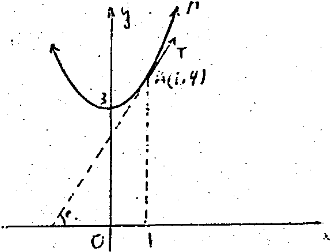
\includegraphics[width=0.25\textwidth]{images/b2p2-296-fig01}

      $y' = 2x |_A = 2 \to tan\alpha = 2$

      $cos\alpha = 1 / \sqrt[]{5}, \ sin\alpha = 2 / \sqrt[]{5}$
      \end{center}
      
    since $\alpha$ is acute. 
    \end{hSolution}	%Solution continues in next page

\end{document}